\section{Introduction}
\label{sec:intro}
Electron micrographs (Fig.~\ref{fig:img} (a)) are obtained by cryo-electron tomography (CET) \cite{Hawkes2007}, which is an advanced technique to visualize the \change{near-to-native} environment of neurones, such as cytosol or lysate and lipid membranes~\cite{Lucic2005a}.
\xj{I can not find anyone using "near-to-native". you use 'native' many times in the draft.}
%
Among all kinds of cellular materials, biological macromolecules in synaptic cleft regions are one of the hottest study areas, as they play an important role in neurotransmitter transmission.
%
In the last decade, it mainly relied on manual segmentation of synaptic cleft regions, which is time-consuming and subjective, to analyze those macromolecules of interest.
%
Our goal in this paper is to develop an automatic approach to automatically extract the accurate region of synaptic cleft from noisy electron micrographs (Fig.~\ref{fig:img} (b)).


%The challenges behind this task are not easy to resolve by existing segmentation methods.
Automatic segmentation of synaptic cleft is challenging in many aspects. 
Firstly, due to the radiation damaging during CET, electron micrographs suffer from a large amount of noise and low signal-to-noise ratio (SNR).
Secondly, the synaptic cleft region is typically a quite small fraction of a high-resolution $2D$ electron micrograph, which requires a high precision of segmenting small objects.
Thirdly, only the cellular cleft, adjacent to one synapse and receiving neurotransmitter molecules from another synapse, is the desired synaptic cleft. This requires the segmentation technique to encode munch \xj{much more global?} biological knowledge for judgement.
Finally, as the most of concerned macromolecules exist on the surface of presynaptic membranes, it puts forward a higher demand on accurate contour localization.

\begin{figure}[t]
    \begin{center}
        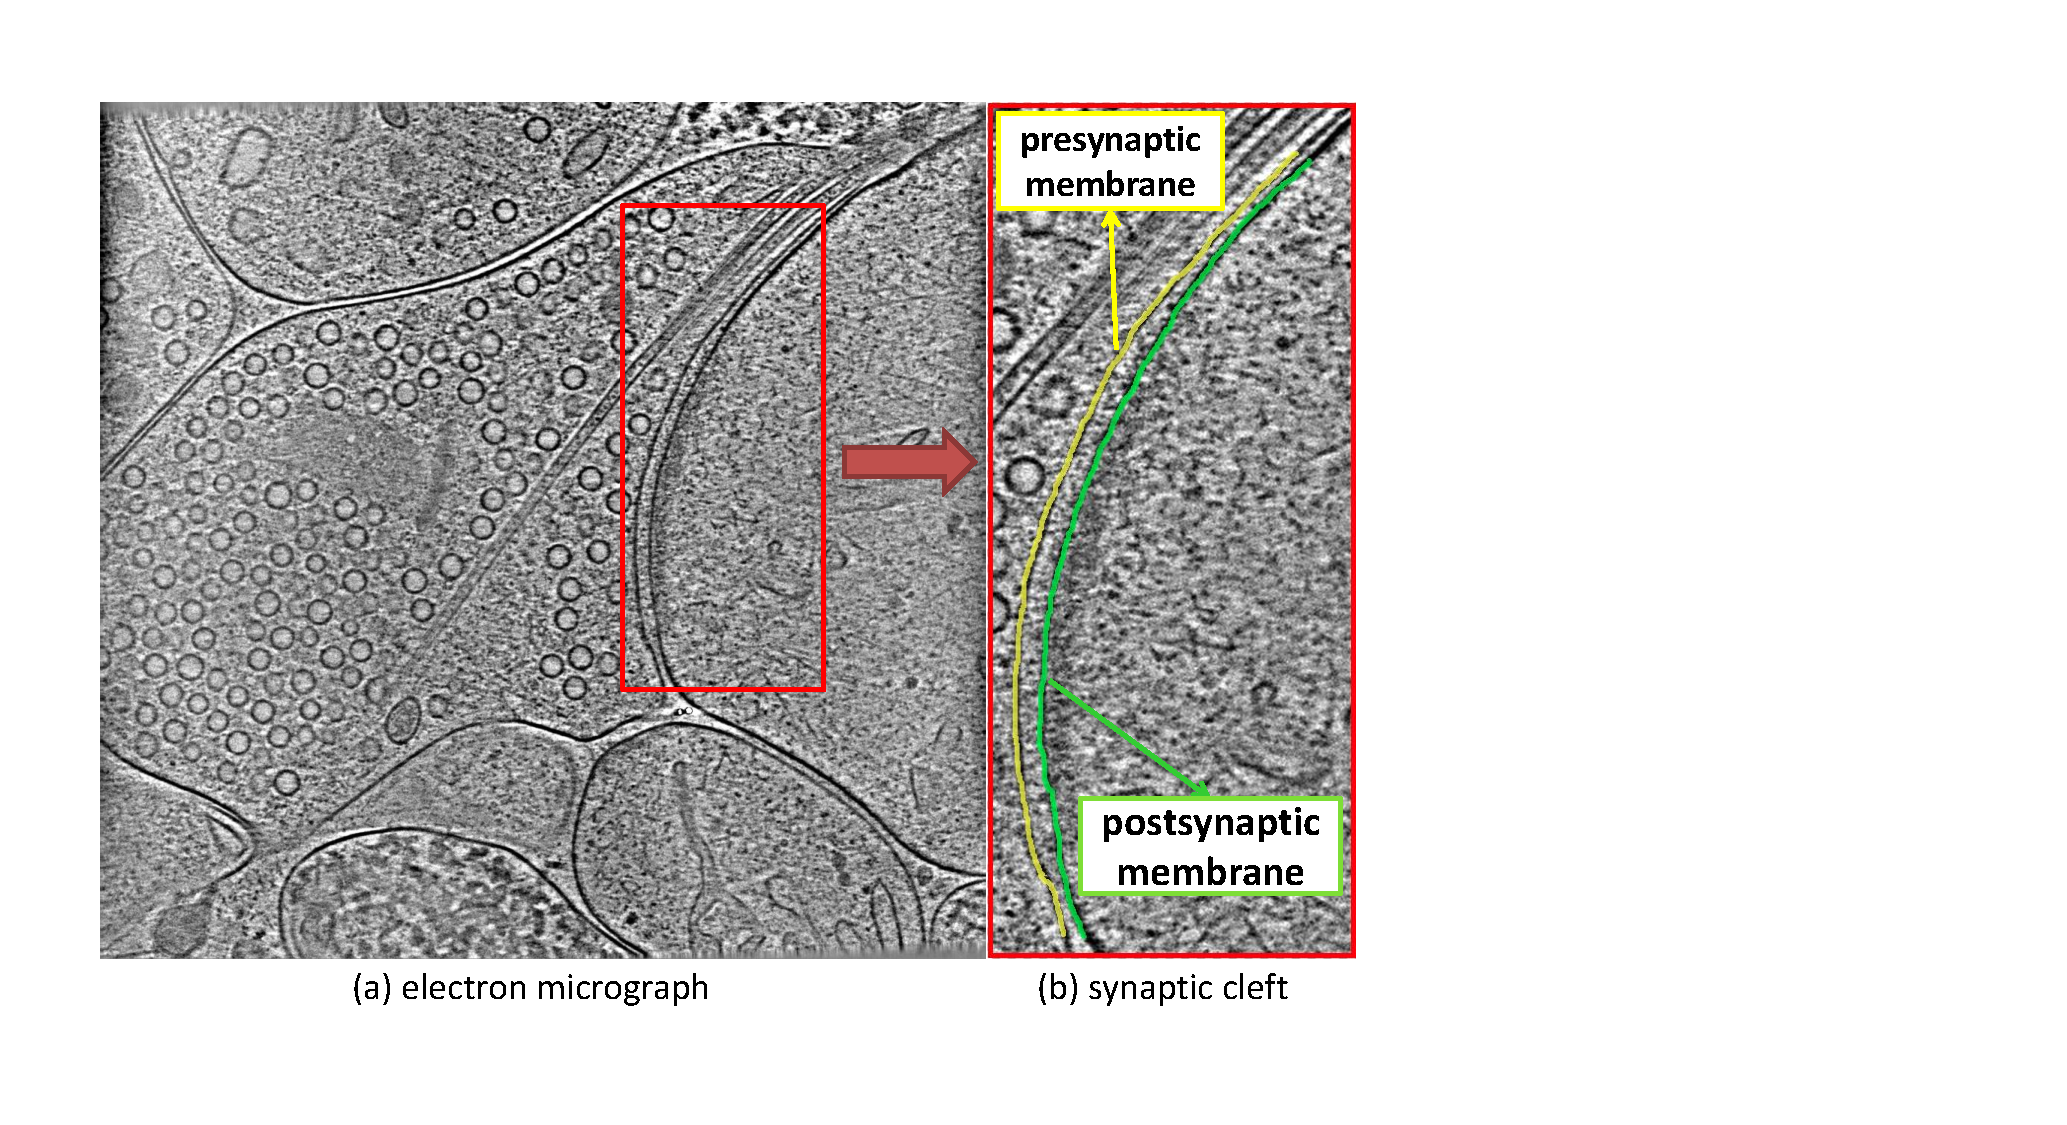
\includegraphics[width=3.4in]{figs/FigImg.pdf}
   \end{center}
\caption{(a) An electron micrograph containing a synaptic cleft region in the red box. 
            (b) Especially, the synaptic cleft region is surrounded by a presynaptic membrane (yellow) and a postsynaptic membrane (green). \xj{emphasize the region with a mask?} }
\label{fig:img}
\end{figure}


Recently, fully convolutional networks (FCN)~\cite{Long2015,Ronneberger2015,Chen2016a,Chen2017,Zhao2016} have achieved great progress in image segmentation, and variants of FCN \cite{Ronneberger2015,Chen2017,Dhungel2015,Lieman-Sifry2017,Chen2016b,Ourselin} show their promising performance in biomedical image processing.
%
The famous U-net~\cite{Ronneberger2015} directly concatenates the features from downsampling to upsampling layers for supplementing low-level information and better contour localization.
Soon, Chen et al.~\cite{Chen2016a} developed the dilated convolution operation by introducing zeros into the original convolutional kernel for lager receptive field and achieved amazing performance in natural image segmentation.
DCAN~\cite{Chen2017} integrates complementary information of objects and contours in a multi-task learning framework to separate the clustered objects into individual ones.
Moreover, PSPNet~\cite{Zhao2016} uses the more powerful ResNet~\cite{He2016} for feature extracting and proposes a pyramid pooling module to better exploit the global context information.
%
Although these techniques have achieved great success in many challenging datasets, they still face challenges when processing electron micrographs, which have unique textures and structures.

\xj{For referennces, use author [ref] proposed a method... or A method is proposed [ref] to ...}

\begin{figure*}[t]
    \begin{center}
        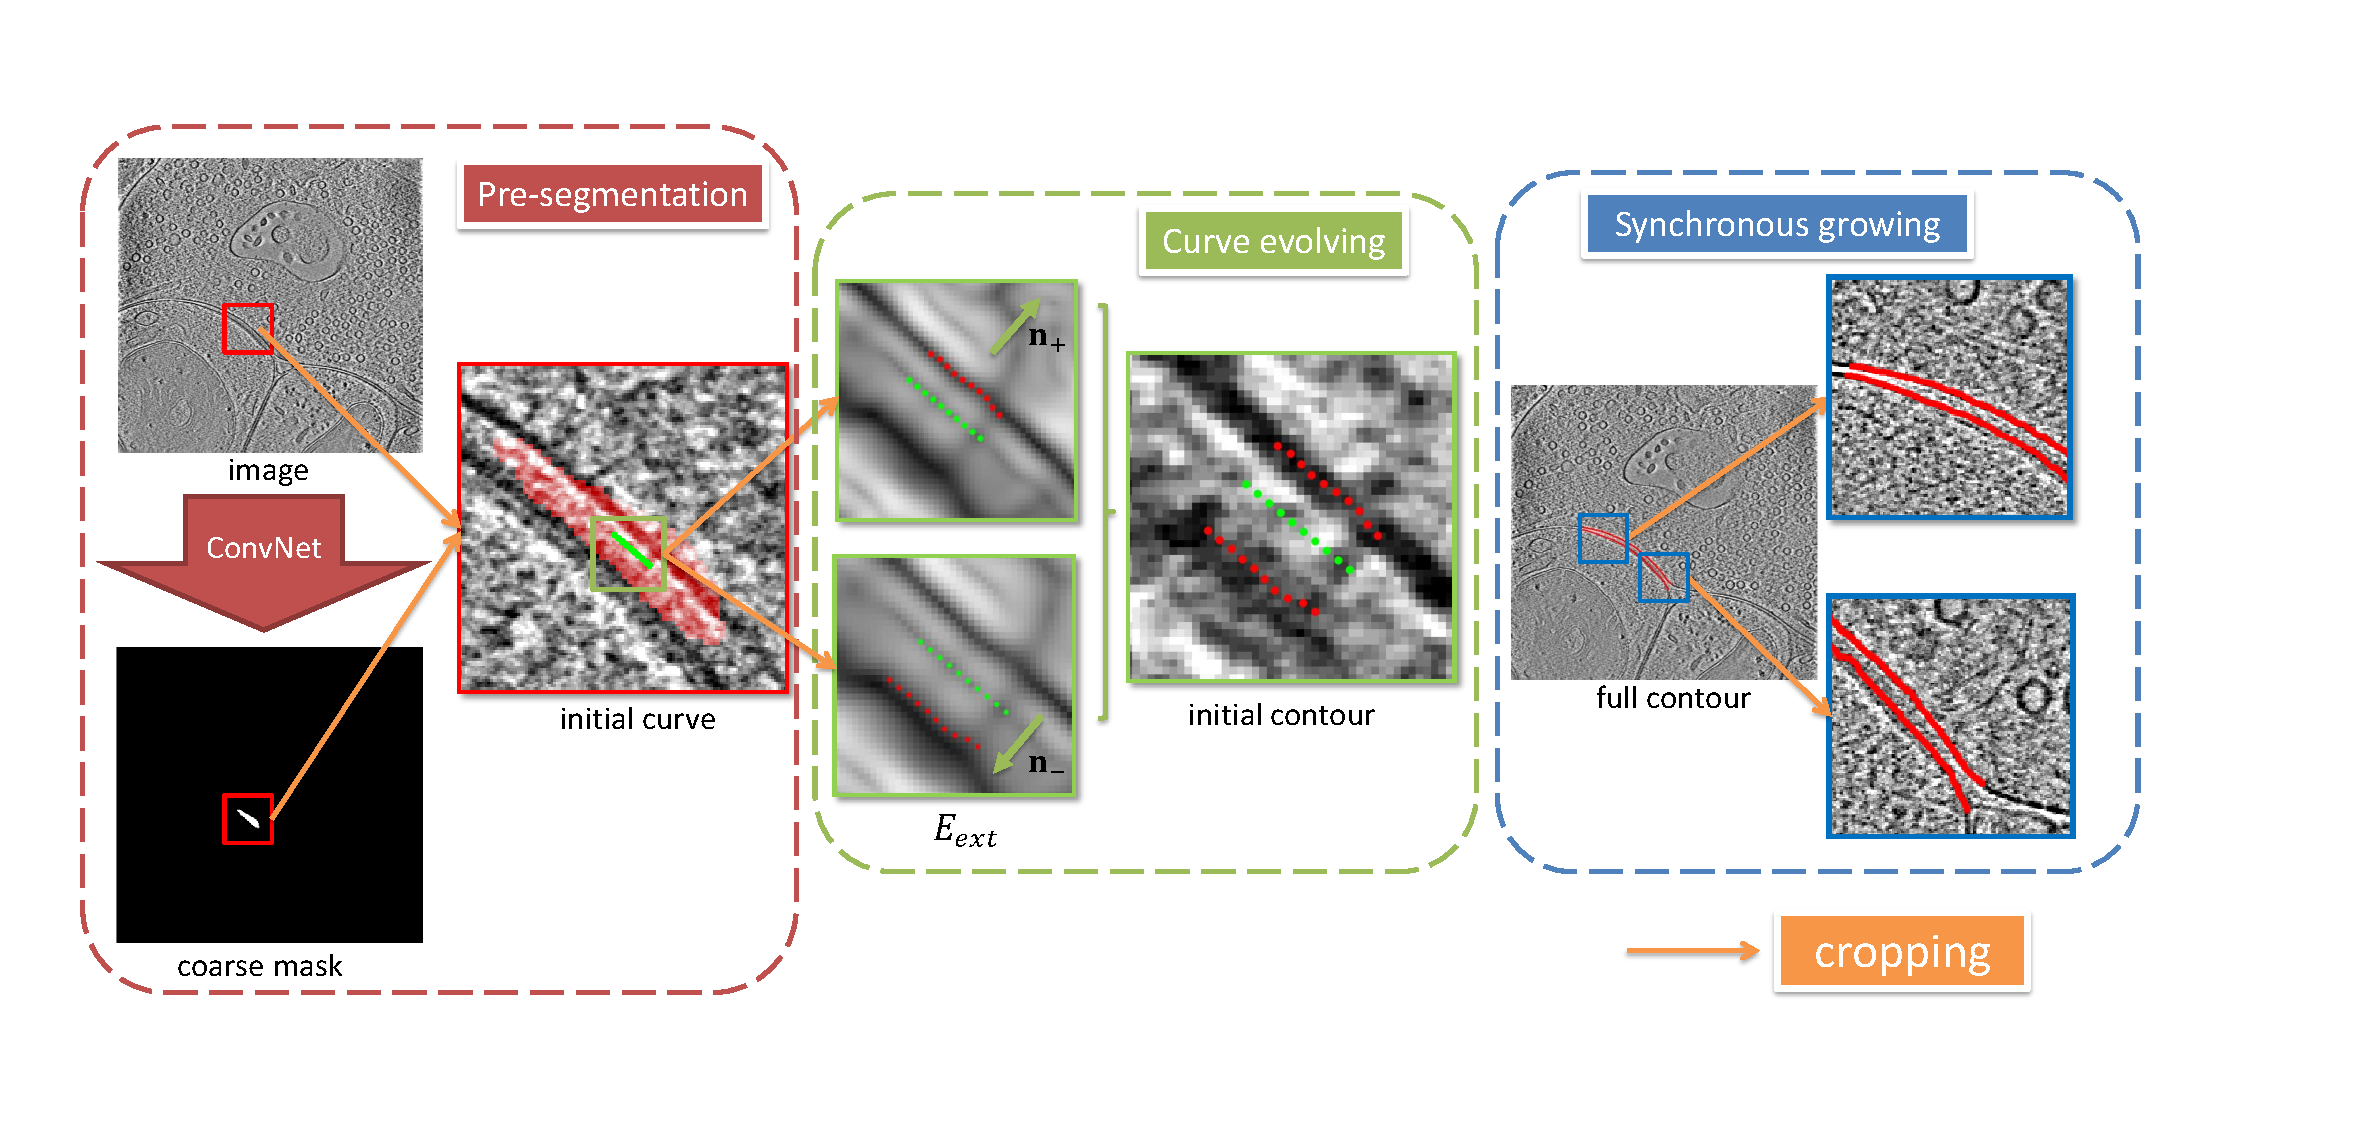
\includegraphics[width=7in]{figs/FigCG.pdf}
   \end{center}
\caption{A brief view of our algorithm in localizing the synaptic cleft region. First a CNN-based model results in a coarse segmentation mask, which provides an initial curve (green line) in cleft region.
        Then, the initial curve is respectively evolved along opposite direction ($\mathbf{n}_+$ and $\mathbf{n}_-$) to obtain two pieces of initial contours (red dotted line).
        Finally, the two contours will synchronously grow to localize the whole synaptic cleft region (encircled by red solid curves).}
\label{fig:cg}
\end{figure*}


Though FCNs have difficulties on extracting precise boundaries for synaptic cleft, our method is built on FCNs, taking their advantages of efficiently localizing the synaptic cleft region in a large-size electron micrograph. 
%
Then a novel contour growing process is concatenated to the FCN to extract accurate contours of the target synaptic cleft region.
%

\comments{
In this paper, we propose an effective framework for segmenting target region in electron micrographs by combining intelligent CNN \xj{{better using FCN?}} and a novel contour growing algorithm.
Our method consists of two main steps.
First, a FCN-based segmentation is employed to coarsely extract the synaptic cleft region. \xj{only one cleft region or mulitple regions?}
%
And then, our contour growing algorithm takes in the segmentation and results in precise contour localizations of target synaptic cleft region.}
The insight of our method is that the contours localized by FCNs are usually poor and unsatisfied, due to successive downsampling layers~\cite{Chen2017}, but it successfully produces an accurate localization of our plausible region.
%
Therefore, we utilize the ability of FCN of learning high-level biological knowledge to globally pick out synaptic cleft regions from such a complex environment.
%

Our contour growing algorithm is robust and efficient, because it is a self-correcting model and uses the local texture information for inference.
With a coarse segmentation of target region, the method first generates a piece of accurate contour from the mask as origin and then gradually grows the whole contours of the target region.
Especially, as long as the major part of initial curve is successfully evolved to target contour, the following growing process will be not affected.
%
However, since the contour of a synaptic cleft is not closed and consists of the presynaptic and postsynaptic membranes as shown in Figure \xj{fig no?}, we should simultaneously grow two piece of contours and decide when the growing terminates according to the distance between these two membranes.


Our main contributions are threefold:
\begin{enumerate}
	\item We propose a new framework to accurately segment the target region in electron micrographs.
	\item A novel updating strategy of active contours is developed, which is more robust and effective.
	\item Specific to segment synaptic cleft region, we propose a algorithm to synchronously grow both two contours.
\end{enumerate}